\section{Understanding the YoungDrive participants}

The following section describes roles, businesses, and coach descriptions for Uganda and Zambia.

\subsection{Roles}

The \textit{country manager} trains the project leaders. It is also the main person responsible for partnerships and the quality of the YoungDrive program in the respective country.

The \textit{project leaders} trains the coaches. They oversees the coaches, manages the coach training, and also collaborates with local stakeholders for quality assurance and to oversee daily operations.

The \textit{coaches} trains the youth. In Zambia, a coach only has responsibility for training youth in the YoungDrive program. In Uganda, this is called a \textit{Youth Mentor}, in contrast to being a \textit{Community Based Trainer (CBT)}, which also trains the youth in other programs and leads the youth saving groups. Most of the CBT's in Uganda holds sessions together with a Youth Mentor, or divides work between them, instead of being alone. The coaches are often volunteers, receiving a small scholarship from the partner organization. They are often business owners themselves. The coaches could be described as social entrepreneurs \citep{mitchel}. Many of the YoungDrive coaches (and youth) are driven by that their business can have an impact on their community, \textit{as well} as take them out of unemployment or increase their current livelihood.

The \textit{youth} are the ones receiving the training from the CBTs and the YMs, being encouraged to start their own businesses.

\subsubsection{Country Managers}

In Uganda, the country manager is Iliana Björling. She is located in the Uganda capital, Kampala, which is a strategic location because it is the same city in which the national office of the main partner, Plan International, is located.

In Zambia, the country manager is Josefina Lönn, who previously was project leader in Kampala, and has held all the trainings up to this point. Now, she leads the operations and has trained the coaches in Zambia, in the new role of country manager and project leader.

\subsection{Social characteristics}

According to statistics gathered by YoungDrive during 2015 evaluations \cite{youngdrive-statistics}, there are a number of considerations to make regarding the coaches in Uganda. This regards entrepreneurship experience, technical access, and language, see a summary in figure \ref{fig:ydStatistics}.

\begin{figure}[h]
    \centering
    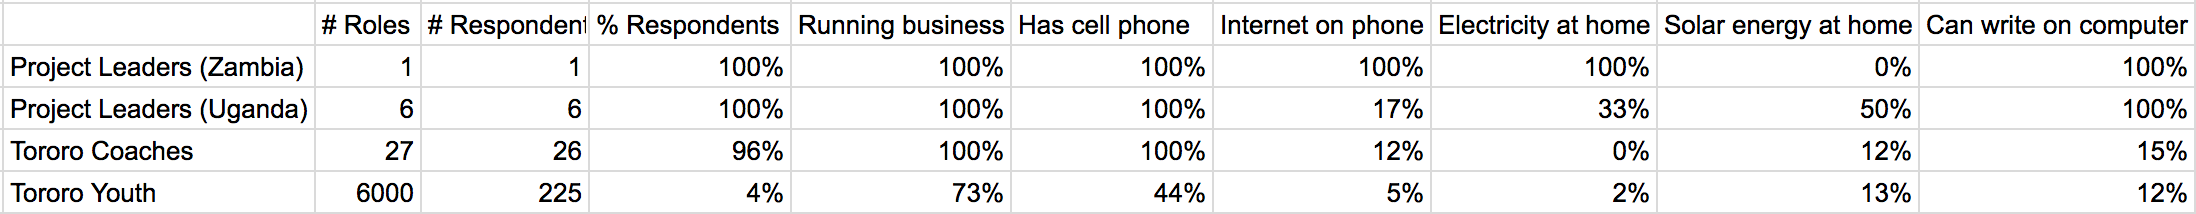
\includegraphics[width=0.7\textwidth]{ydStatistics.png}
    \caption{Table showing entrepreneurship experience, technical access, and language between coaches and project leaders in Uganda and Sambia.}.
    \label{fig:ydStatistics}
\end{figure}

All of the Tororo coaches run a business (26/26 respondents), with a majority running more than one. This means, they do have practical experience of running a business outside of the YoungDrive coach training.

While all have a cell phone, smartphones are very uncommon - only 3 uses Internet on the phone, every day or weekly, mostly for Facebook or email. Regarding power, none (0/26) has power at home, 3/26 has solar, and only 4 can write on a computer. Taken together this means that their technical skills are low, and needs to be in consideration.

Regarding language, English can be used in the coach app. While about half of the asked Uganda youth can not understand (129/225), read (133/225) or write (132/225) English, most of the coaches in Uganda are proficient.

These characteristics can be used for youth and project leaders as well.

\subsection{Tororo businesses}

The coaches in Tororo are divided into three different regions. Based on region, income and experience, they run different kinds of businesses. \footnote{In Uganda and Zambia, a small-scale business is typically not registered. Thus, the coaches' definition of a business can be more generous.}

In Tororo, the coaches' businesses range from: ananas, water melon, onion, chili, bakery, catering, corn, beans, fabric, plastic products, bird farm, milk, fish, ground nuts, cabbage, tomato, hairdresser, sewer, shop and rice. For reference of environment, see figure \ref{fig:tororo}.

\begin{figure}[h]
    \centering
    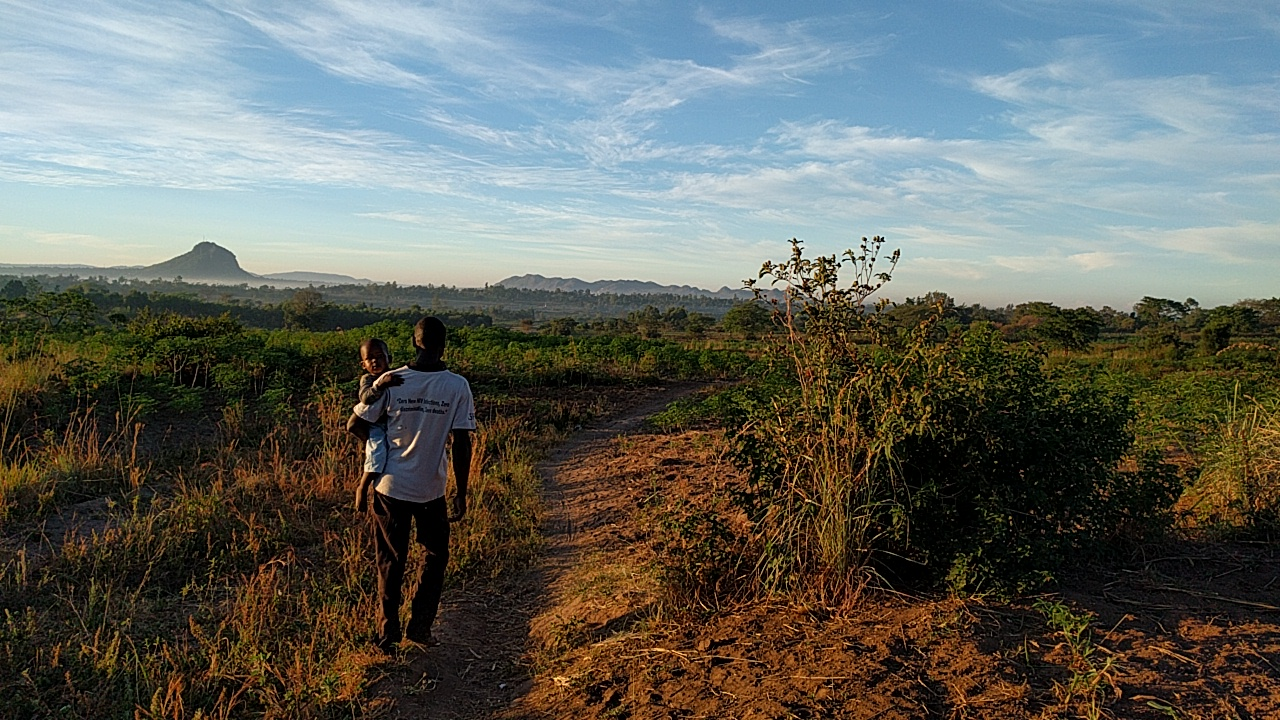
\includegraphics[width=0.7\textwidth]{stayover.jpg}
    \caption{Local project leader Patrick showing the rural part of Tororo, where crops are growing close to where he lives.}.
    \label{fig:duolingo}
\end{figure}

In Tororo, there are 2 Project Leaders. Christine's business ranges from: bakery, corn, pig farm and plastic products. Patrick's business ranges from: silver fish, beans, corn, and bird farm. In comparison, in Kamuli, there are 4 Project Leaders. Their businesses ranges from: selling office supply, boda boda, bird farm, pig farm, green pepper, corn, cabbage, tomate, aubergine, chipati ("bread"), chilli, and charging of cellphones.

Among the youth, the top 8 most popular businesses in Tororo, with 134 respondents, are corn, cassava ("potato"), saloon, fish, making of bricks, beans, brooms and rope. These range from 9 for corn (6.7\%) to 5 for rope (3.7\%).

\subsection{Zambia coaches}
The Zambia coaches in Kabwe are better educated, and have better access to technology, compared to the ones in Uganda. Regarding sociology, ages ranged from 21-39 years old (26.8 average). 3 were mentioned as being shy during the interviews. They lived from 10-90 minutes outside of town (33 minutes average).

Regarding motivations for being a coach, 50\% had an emphasis on benefiting the community, and 90\% had personal reasons. The following statistics has been derived from the notes of the Zambian coach job interviews \cite{yd-zambia-interviews}.

%Care for oneself:
%\begin{itemize}
%\item Learn business %(7)
%\item More skills %(2)
%\item Get idea
%\item Expand business
%\item Benefit CV
%\end{itemize}
%
%Care for community:
%\begin{itemize}
%\item Empower %(2)
%\item Teach business
%\item Leadership
%\item Share
%\item Stop bad behaviours of youth
%\end{itemize}

Regarding experience, 8 had trained youth before, 8 had been a leader before, 9 had business experience.

Regarding YoungDrive, they said they could handle training between 8-30 youth (19.8 on average) per group. They could have 1-5 groups per coach (average 3.0), totalling a range between 8-101.5 youth (average 59.8).

During the visit in Zambia, the coaches had not yet formed their youth groups, and started their own sessions.
